\documentclass{../bredelebeamer}
\usepackage{multirow}
\usepackage{pdfpages}
\usepackage{braket,bigstrut}
\usepackage{palatino}
\usepackage{multicol,bigstrut}
\usepackage{listings}
\usepackage{tikz}
\usepackage{pgfplots}
\pgfplotsset{compat=1.17}
\usepackage{booktabs}
\usepackage{amsmath,amssymb,amsfonts,cancel,physics,siunitx}
\usetikzlibrary{positioning,shadows,backgrounds,calc}%
\setbeamercolor{footnote mark}{fg=black}
\setbeamercolor{footnote}{fg=black}


\renewcommand{\baselinestretch}{0.9}

\usepackage[backend=bibtex8,style=authortitle,autocite=footnote]{biblatex}
%\addbibresource{../../references.bib}

\renewbibmacro*{cite:title}{%
	\printtext[bibhyperref]{%
		\printfield[citetitle]{labeltitle}%
		\setunit{\space}%
		\printtext[parens]{\printdate}%
	}%
}

\renewcommand{\figurename}{{\bf Fig.}}
\usefonttheme{serif} % default family is serif

\renewcommand{\baselinestretch}{0.9}

\title[Ditaus - COMHEP 2024]{
	{\huge
	On the Effects of Interference in BSM Production and Detection of $\tau\tau$ at the LHC
	}
}
\subtitle{}
\author[Cristian F. Rodríguez C.]{%
	{\Large
		$ $\\
		Cristian Fernando Rodríguez Cruz\\
		$ $\\
		$ $\\
		Authors:\\
		A. Flórez\inst{1}, \textcolor{Framableu}{\textbf{C. Rodriguez}}\inst{1}, J. Reyes-Vega\inst{1},\\
		J. Jones-Pérez\inst{2}. \\
	}
}
\institute[Uniandes]{%
	{\large
		\inst{1} Universidad de los Andes\and
		\inst{2} Pontificia Universidad Católica del Perú
	}
}
\date{\today}
\lstset{language=C++,
  basicstyle=\ttfamily,
  keywordstyle=\color{blue}\ttfamily,
  stringstyle=\color{red}\ttfamily,
  commentstyle=\color{green}\ttfamily,
  morecomment=[l][\color{magenta}]{\#}
}

\begin{document}
\frame{\titlepage}

\begin{frame}
    \frametitle{Outline}
    \tableofcontents
\end{frame}

\section{Introduction}
\subsection{Motivation}
\begin{frame}{The Standard Model of Particle Physics}
    \begin{minipage}[t]{0.43\linewidth}
        Weak bosons mix the different generations of quarks via the CKM matrix, but this does not happen for leptons. This property of the model is known as \textbf{lepton flavor universality (LFU)}.

        \begin{center}
            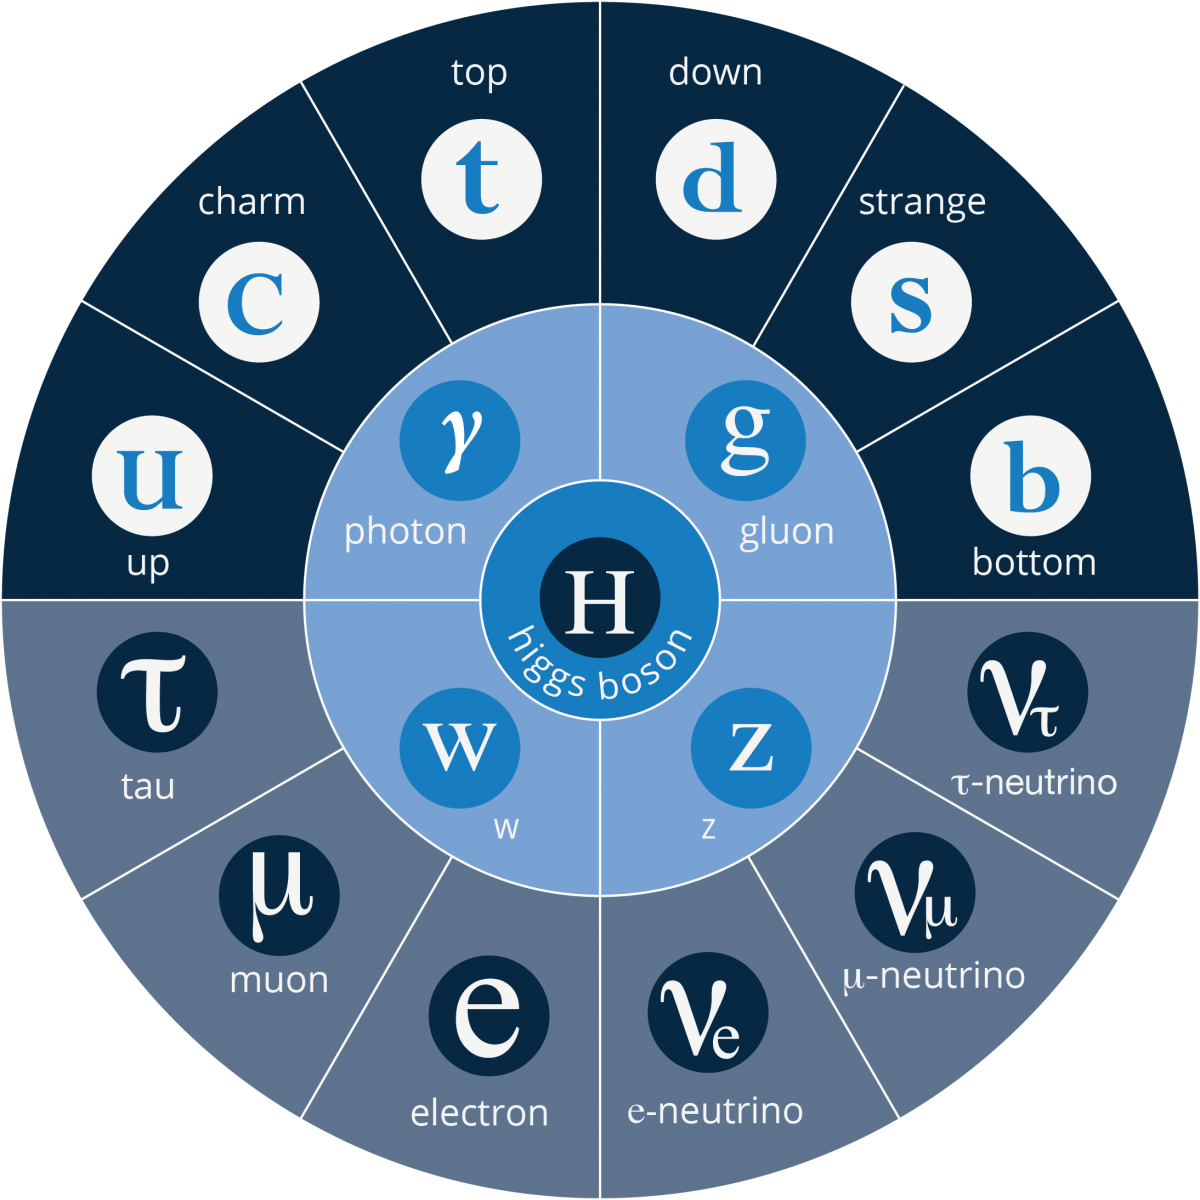
\includegraphics[width=.9\linewidth]{SM}
        \end{center}

    \end{minipage}
    \hfill
    \pause
    \begin{minipage}[t]{0.53\linewidth}
        %\centering

        However, recent measurements of the $R(D)$ and $R(D^*)$ ratios show a deviation from the SM predictions. This could be a hint of \textbf{lepton flavor violation (LFV)} and then  \textbf{new physics beyond the SM}.

        $$ $$

        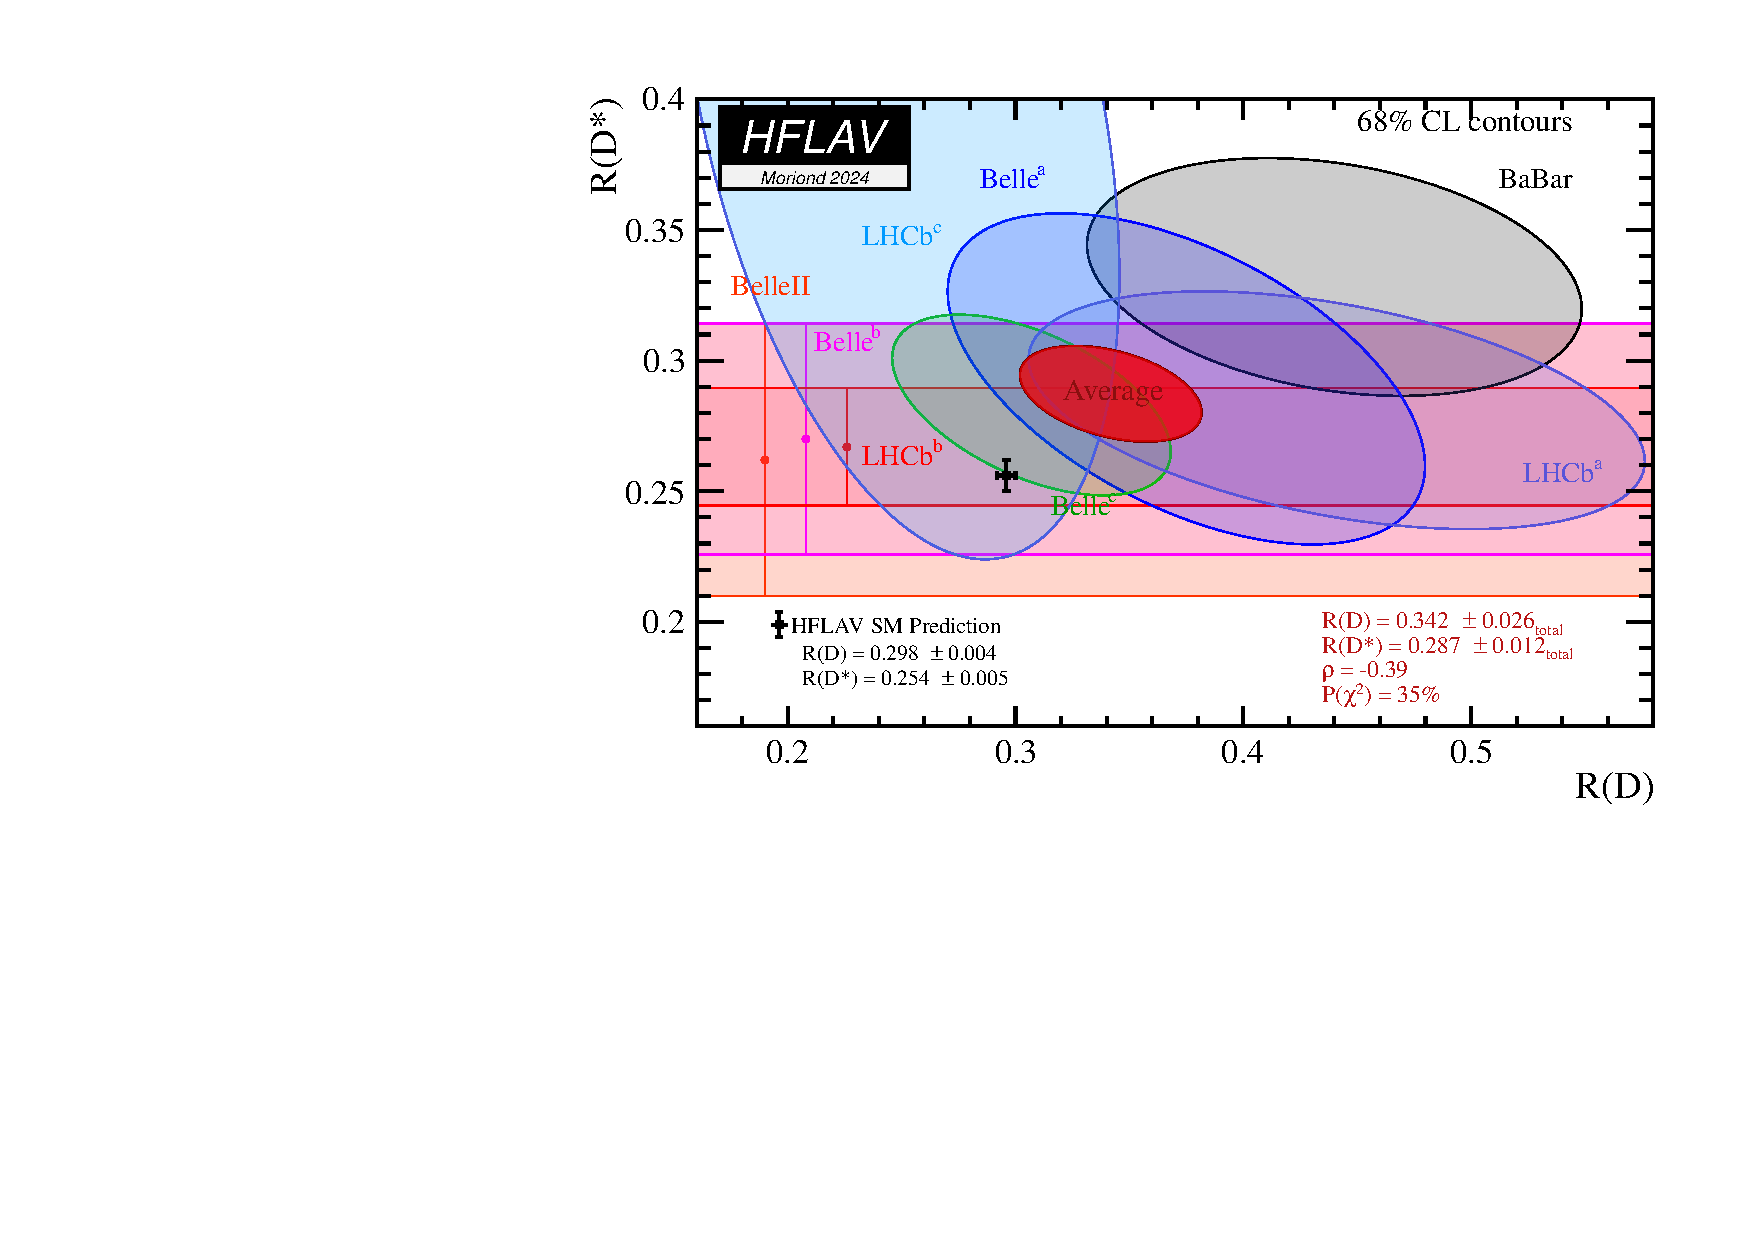
\includegraphics[width=1.05\linewidth]{../2023_paper/RDRDst_hflav.pdf}    
    
    \end{minipage}
\end{frame}

\begin{frame}{Large Hadron Collider}
	\begin{minipage}{.55\linewidth}
		{\centering
		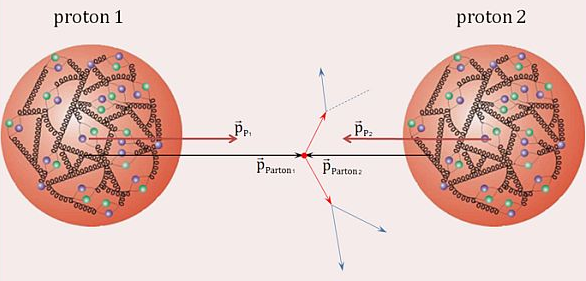
\includegraphics[width=.9\linewidth]{pp_collision.png}
		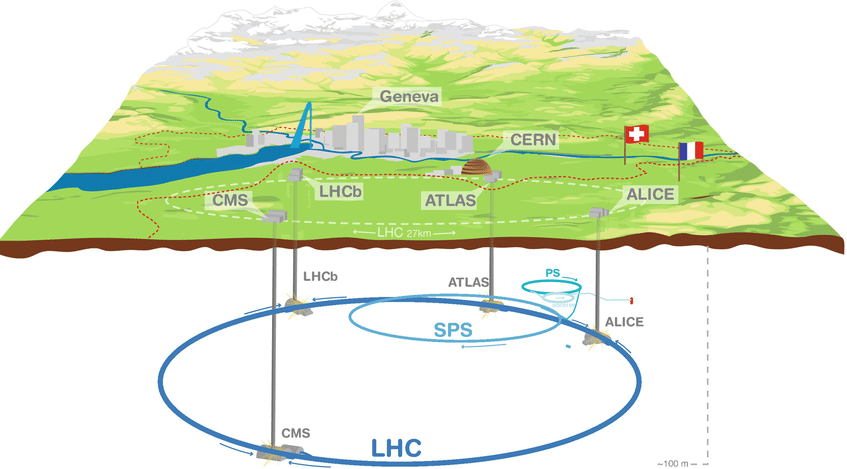
\includegraphics[width=.99\linewidth]{../2023_paper/LHC.png}
		}
	\end{minipage}
	\pause \hfill
	\begin{minipage}{.42\linewidth}
		\begin{itemize}
			\item Feasibility Studies is needed.
			$$ $$
			\item Take Care on the dependence on the different parameters.
			$$ $$
			\item Take care on the content of particles.
			$$ $$
			\item Take care of the signal composition.
			$$ $$
			\item Take care on interference effects.
		\end{itemize}
	\end{minipage}
\end{frame}

\subsection{BSM Signatures}
\begin{frame}{BSM Signatures on the Di-Tau Channel at the LHC}{LFV and $\tau$ lepton as window to new physics}
	%Assuming that the LFV can be explained models which have a preferential coupling to the third generation of fermions, we can explore the structure of that models by studying the di-tau channel at the LHC.
	
	In the different models, we can have different production mechanisms. 
	
	For example, resonant ones

	\begin{minipage}{.45\linewidth}
		\begin{center}
			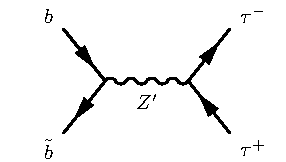
\includegraphics[width=.9\linewidth]{DY.pdf}
		\end{center}
	\end{minipage}
	\hfill
	\begin{minipage}{.45\linewidth}
		\begin{center}
			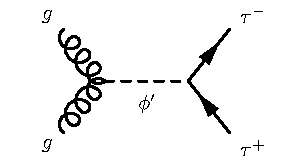
\includegraphics[width=.9\linewidth]{DY_scalar.pdf}
		\end{center}
	\end{minipage}
	
	\vfill%\hrule\vfill
	or non-resonant ones

	\begin{minipage}{.45\linewidth}
		\begin{center}
			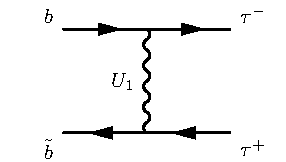
\includegraphics[width=.9\linewidth]{non-res_vector.pdf}
		\end{center}
	\end{minipage}
	\hfill
	\begin{minipage}{.45\linewidth}
		\begin{center}
			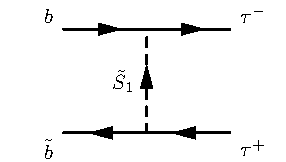
\includegraphics[width=.9\linewidth]{non-res_scalar.pdf}
		\end{center}
	\end{minipage}
  \begin{center}
		{ \large
		Different Models could have one or several contributions to the di-tau channel, and the \textbf{interference between them could be relevant.}
		}
	\end{center}
\end{frame}


\subsection{Interference Phenomena in the SM}
\begin{frame}{Interference Phenomena in the SM}{Photon and $Z$-boson interference, $q \bar q \longrightarrow \tau^+ \tau^- $}
    
    \begin{minipage}{0.65\textwidth}
        The squared matrix element can be written as
        \begin{equation}
            \begin{aligned}
                \abs{\mathcal{M}}^2 & =\abs{\mathcal{M}_{\gamma^*}+\mathcal{M}_{Z}}^2
                \\&= \abs{\mathcal{M}_{\gamma^*}}^2 + \abs{\mathcal{M}_{Z}}^2 + 2\Re\left( \mathcal{M}_{\gamma^*}^*\mathcal{M}_{Z} \right).    \notag
            \end{aligned}
        \end{equation}
    \end{minipage}
    \hfill
    \begin{minipage}{0.33\textwidth}
        \begin{center}
            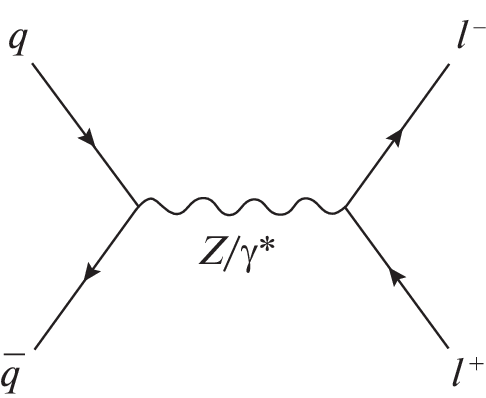
\includegraphics[width=.8\linewidth]{DY.png}
        \end{center}
    \end{minipage}
    \pause
    $ $\\$ $\\$ $

    For the case $q_R \bar q_L \longrightarrow \tau_L^+ \tau_R^-$, the amplitudes are
    \begin{minipage}{0.65\textwidth}
        \begin{equation}
            \begin{aligned}
                \abs{\mathcal{M}_{\gamma^*}}^2          & = e^4\left[Q^{(f)} Q^{(q)}\right]^2\left[1+\cos \theta\right]^2                                                                      \\
                \abs{\mathcal{M}_{Z}}^2                 & = \frac{s^2 g_Z^4\left[g_R^{(f)} g_R^{(q)}\right]^2}{\textcolor{red}{\left(s-m_Z^2\right)^2+\left(m_Z \Gamma_Z\right)^2}}\left[1+\cos \theta\right]^2 \\
                \mathcal{M}_{\gamma^*}^*\mathcal{M}_{Z} & = \frac{g_Z^2 e^2 Q^{(f)} Q^{(q)} g_R^{(f)} g_R^{(q)}}{\textcolor{blue}{\left(s-m_Z^2+i \Gamma_Zm_Z\right)}} \textcolor{blue}{s}\left(1+\cos \theta\right)^2 \notag
            \end{aligned}
        \end{equation}
    \end{minipage}
    \hfill
    \begin{minipage}{0.33\textwidth}
        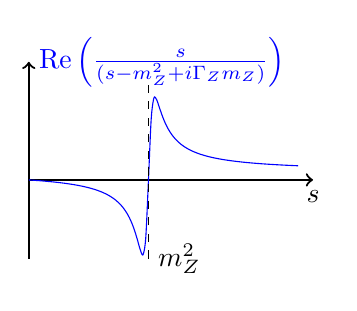
\begin{tikzpicture}[xscale=0.38, yscale=0.1]
            \draw[thick,->] (0,0) -- (9.5,0) node[below] {$s$};
            \draw[thick,->] (0,-10) -- (0,15) node[right,blue] {$ \Re\left(
                    \frac{s}{(s-m_Z^2+i \Gamma_Z m_Z)}
                    \right)$};

            % plot -(m^2 x)/((-m^2 + x)^2 + Γ^2) + x^2/((-m^2 + x)^2 + Γ^2), m=2, Γ=0.2
            \draw[domain=0:9,samples=100,smooth,variable=\x,blue]
            plot ({\x},{-(4*\x)/((4-\x)^2 + 0.04) + \x^2/((4-\x)^2 + 0.04)});
            % put a mark in s=m^2
            \draw[dashed] (4,-10) node[right] {$m_Z^2$} -- (4,12);
        \end{tikzpicture}
    \end{minipage}\pause
		\begin{center}
			{ \large
			Always that you have two or more contributions to a process, the interference between near to the resonances could be relevant.
			}
		\end{center}
\end{frame}    











\section{Example: The $4321$-Model}
\subsection{The model}

\begin{frame}{Example: The Vector Leptoquark Model}
		\begin{center}
			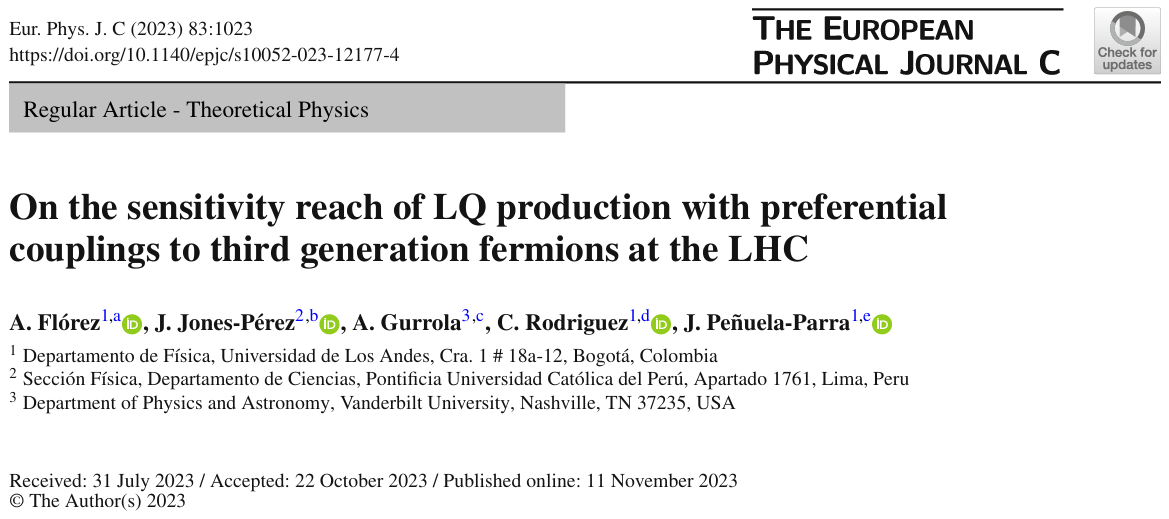
\includegraphics[width=1.03\linewidth]{on_vLQ.png}
		\end{center}	

		\vfill 
		DOI: \href{https://doi.org/10.1140/epjc/s10052-023-12177-4}{10.1140/epjc/s10052-023-12177-4}, 
		
		ARXIV: \href{https://arxiv.org/abs/2307.11070}{2307.11070 [hep-ph].}
\end{frame}

% \begin{frame}{Leptoquarks and $R(D)$/ $R(D^*)$ anomalies}
% 	\begin{multicols}{2}
% 		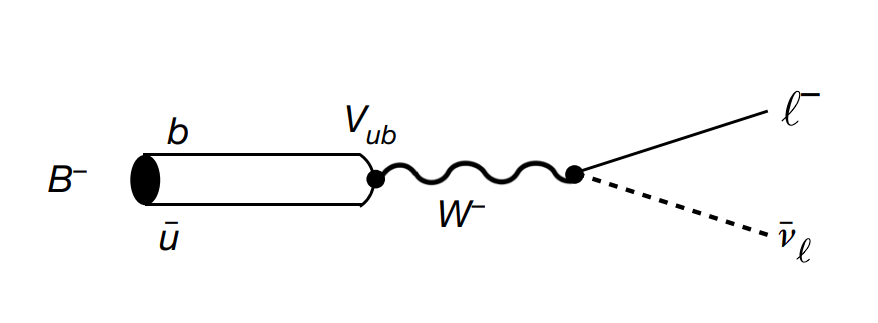
\includegraphics[width=.99\linewidth]{../2023_paper/B_SM_1.png}
% 		$$ $$
% 		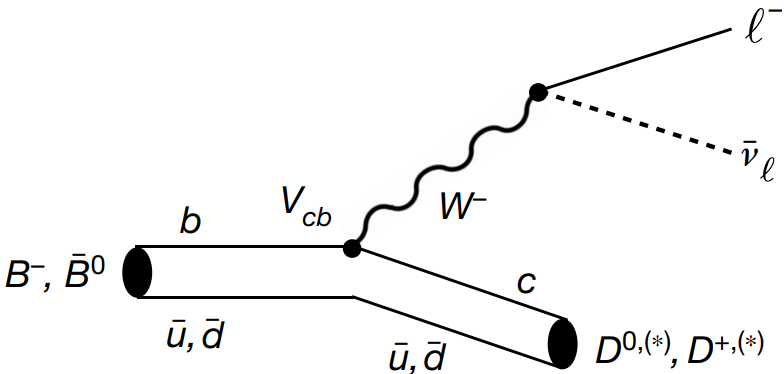
\includegraphics[width=.99\linewidth]{../2023_paper/B_SM_2.png}
% 		\pause
% 		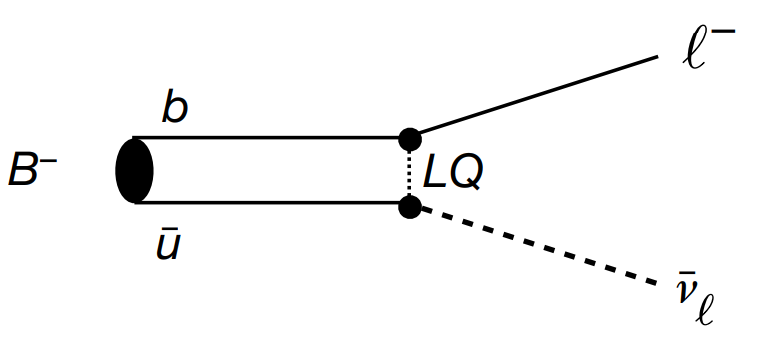
\includegraphics[width=.99\linewidth]{../2023_paper/B_LQ_1.png}
% 		$$ $$
% 		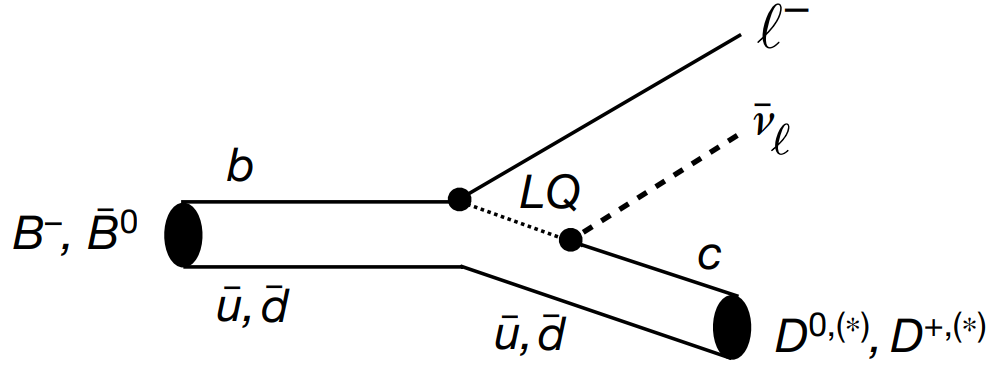
\includegraphics[width=.99\linewidth]{../2023_paper/B_LQ_2.png}
% 	\end{multicols}
% 	\pause
% 	\begin{center}
% 		{\large $ $\\
% 		How can we test this hypothesis?
% 		}
% 	\end{center}
% \end{frame}

\begin{frame}{Example: The Vector Leptoquark Model}
    \begin{multicols}{2}
        A leptoquark is defined as a particle with a vertex that mix vectors and quarks.
        \begin{center}
        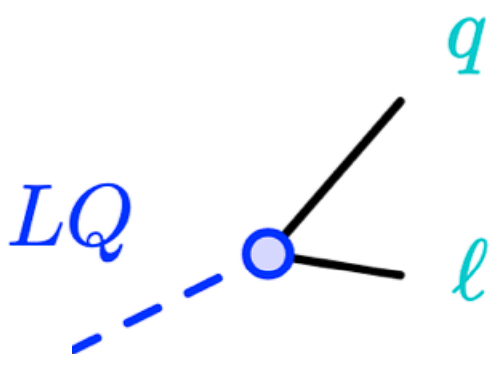
\includegraphics[width=.25\textwidth]{../2023_paper/LQ_vertex.png}
        \end{center}
        If $U_1$ is a vector leptoquark that preserves the chirality on the vertex, we expect an interaction term like
        $$
        \sim U_1^\mu\bar{q}_{L} \gamma_{\mu} \ell_{L},
        $$
        and these allows a similar interaction term for the right handed currents 
        $$
        \sim U_1^\mu\bar{d}_{R} \gamma_{\mu} e_{R}.
        $$
    
        \end{multicols}
        Where the SM charges for the leptoquark, in the $Y=2(Q-T_3)$ convention, are
        \begin{center}
            \begin{tabular}{|c|c|c|c|c|}
                \hline & $\bar{q}_{L}$ & $\ell_{L}^{j}$ & $\bar{q}_{L}\gamma_{\mu} \ell_{L}$ & $U_{1}^{\mu}$ \\
                \hline$U(1)$ & $-1 / 3$ & $-1 $ & $-4 / 3$ & $+4 / 3$ \\
                \hline $\mathrm{SU}(2)$ & $\overline{\mathbf 2}$ & $\mathbf{2}$ & $\mathbf{1}$ & $\mathbf{1}$ \\
                \hline $\mathrm{SU}(3)$ & $\overline{\mathbf 3}$ & $\mathbf{1}$ & $\overline{\mathbf3}$ & $\mathbf{3}$ \\
                \hline
            \end{tabular}	
        \end{center}
        Then, the leptoquark $U_1 \sim \left(\mathbf{3}_{C}, \mathbf{1}_{I}, 4 / 3_{Y}\right)$, and its covariant derivative is
        $$
        \mathcal{D}_\mu U_\nu = \left(\partial_\mu+i g_s T^a G_\mu^a+ i \frac{2}{3} g' B_\mu \right)U_\nu.
        $$
\end{frame}



\begin{frame}{The Vector Leptoquark Lagrangian}
	
	The full Lagrangian for the vector leptoquark is
	\begin{align*}
		\mathcal{L}_{U}=&-\frac{1}{2} U_{\mu \nu}^{\dagger} U^{\mu \nu}+M_{U}^{2} U_{\mu}^{\dagger} U^{\mu}\\&-i g_{s}\left(1-\kappa_{c}\right) U_{\mu}^{\dagger} T^{a} U_{\nu} G^{\mu \nu}_a -\frac{2 i}{3} g'\left(1-\kappa_{Y}\right) U_{\mu}^{\dagger} U_{\nu} B^{\mu \nu}\\
		&+\frac{g_{U}}{\sqrt{2}}\left[U_{1}^{\mu}\left(\beta_{L}^{i j} \bar{q}_{L}^{i} \gamma_{\mu} e_{L}^{j}+\beta_{R}^{i j} \bar{d}_{R}^{i} \gamma_{\mu} e_{R}^{j}
		%+\beta_{N}^{i} \bar{u}_{R}^{i} \gamma_{\mu} N_{R}
		\right)+\text { h.c. }\right]
	\end{align*}
	where $U_{\mu \nu}=\mathcal D_{\mu} U_{\nu}-\mathcal D_{\nu} U_{\mu}$, $\mathcal D_{\mu}=\partial_{\mu}-i g_{s} G_{\mu}^{a} T^{a}-i \frac{2}{3} g_{Y} B_{\mu}$, and the couplings $\beta_{L}$ and $\beta_{R}$ are complex $3 \times 3$ matrices in flavor space. 
	
	\pause \vfill
	
	The $\Delta F=2$ and constrains on lepton flavor violating processes indicates an structure as 
	\begin{equation*}
		\beta_L=\left(\begin{array}{ccc}
			0 & 0 & \beta_L^{13} \\
			0 & 0 & \beta_L^{23} \\
			0 & \beta_L^{32} & \beta_L^{33}
			\end{array}\right), \quad \beta_R=\operatorname{diag}\left(0,0, \beta_R^{33}\right)
	\end{equation*}
	
	If $U_1$ has a gauge origin $\kappa_{c}=\kappa_{Y}=0$. We choose $U(2)$ in quark and leptons space, in a way that you have an hierarchy, $\left|\beta_L^{31}\right| \ll\left|\beta_L^{23}\right|,\left|\beta_L^{32}\right| \ll\left|\beta_R^{33}\right|,\left|\beta_L^{33}\right|=\mathcal{O}(1)$.
	
\end{frame}


% \begin{frame}{Montecarlo Generators}
	

% 	\begin{center}
% 		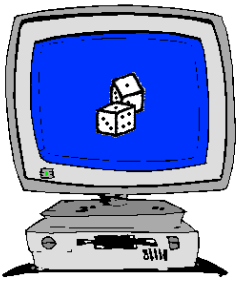
\includegraphics[scale=0.5]{../2023_paper/A1}
% 	\end{center}

% 	Useful to predict what we expect to see under certain conditions:
% 	\begin{itemize}
% 		\item To perform studies before having the data
% 		\item To compute event selection efficiency/acceptance
% 		\item  To predict the ammount and composition of background events
% 		\item To distinguish different signals. 
% 	\end{itemize}
	
% \end{frame}

\begin{frame}{Feasibility Studies Workflow}
	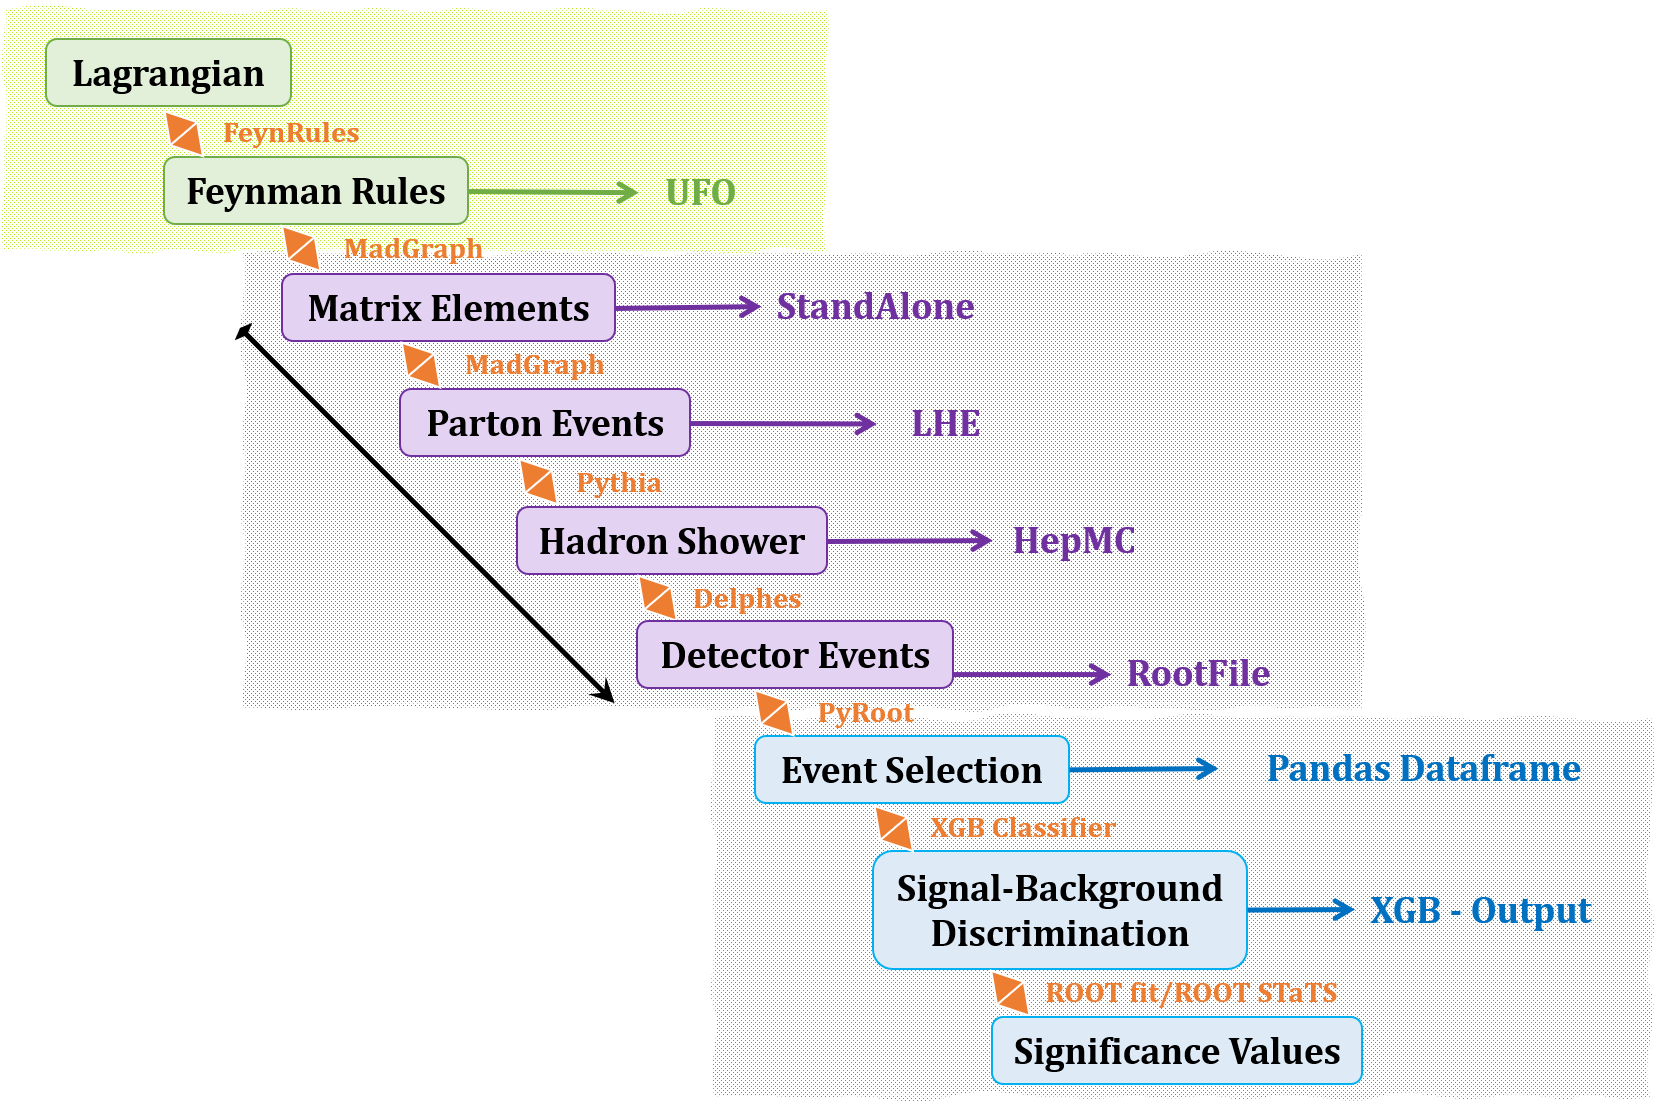
\includegraphics[width=1.0\linewidth]{../2023_paper/Workflow.png}
\end{frame}


\subsection{Sensitivity Reach of the $U_1$ Leptoquark}

\begin{frame}{Sensitivity Reach of the $U_1$ Leptoquark}{$S_T^{\text{meT}}=\left|\va p_{T}^{\,\text{miss}}\right| + \sum_i\left|\va p_{T}^{\,i}\right|$}
	\begin{minipage}{.43\linewidth}
			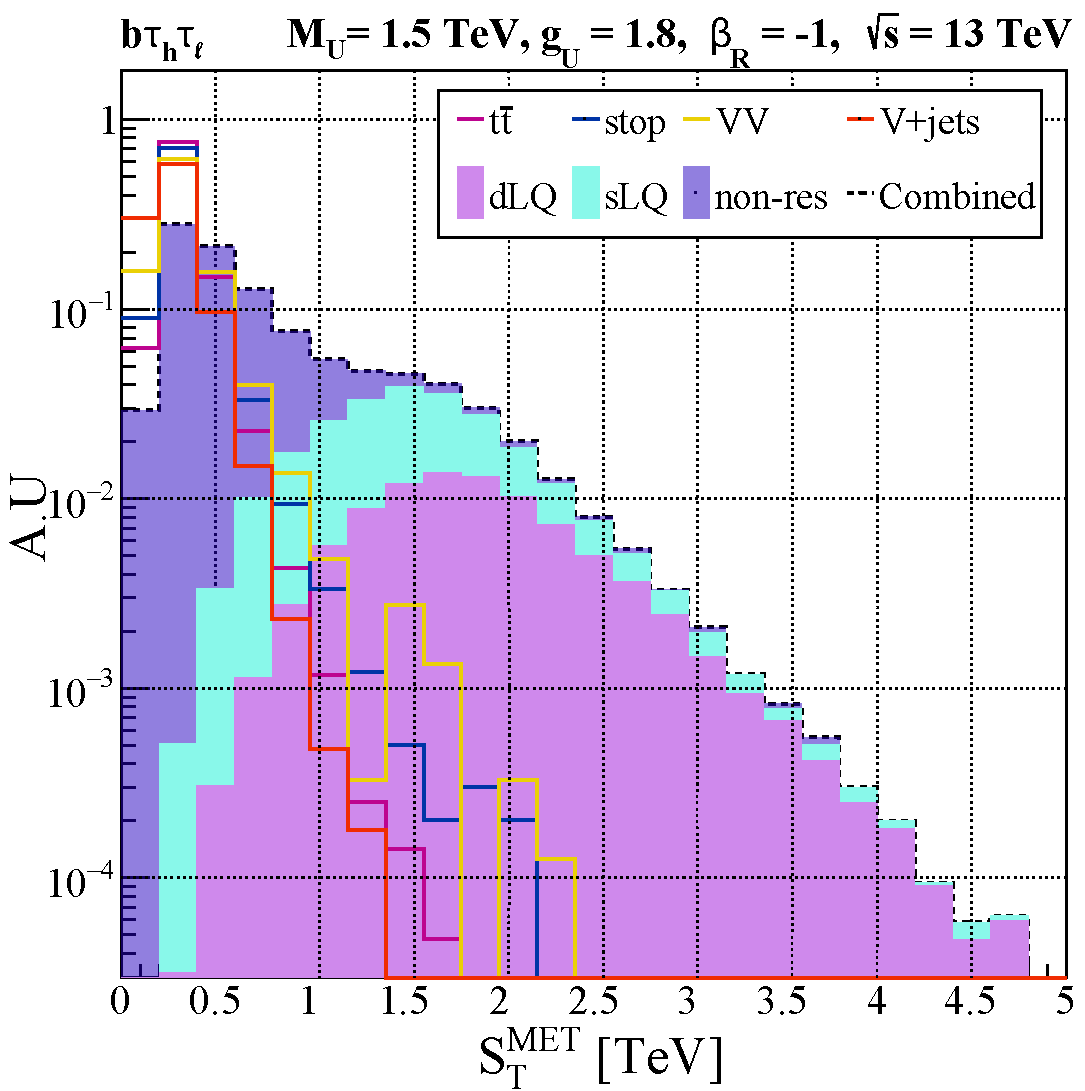
\includegraphics[width=\linewidth]{../2023_paper/sTTeV_semileptonic_sLQ_wRHC.pdf}

	\end{minipage}
	\begin{minipage}{.56\linewidth}
		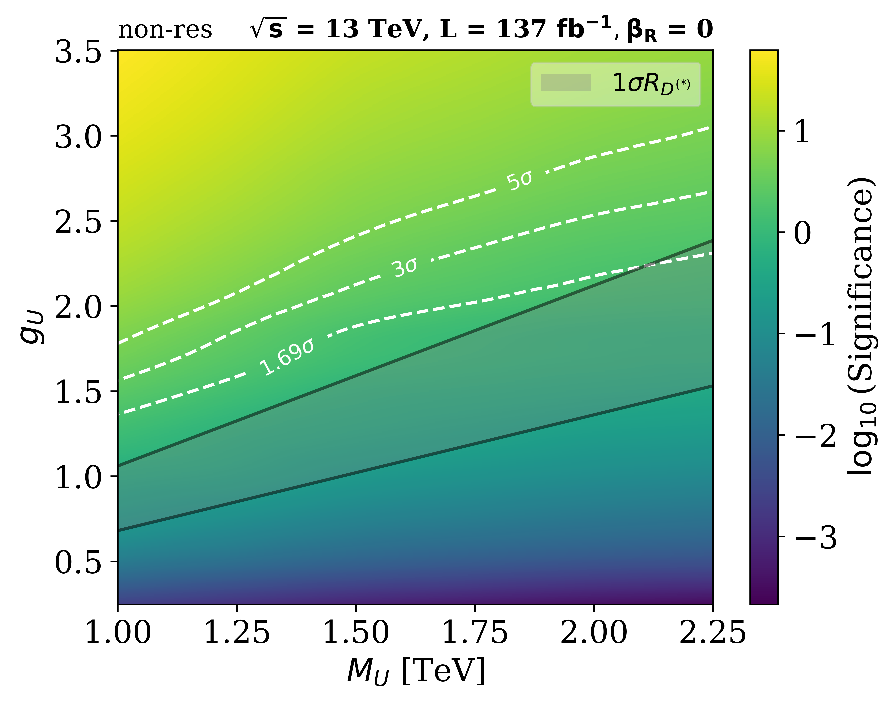
\includegraphics[width=\linewidth]{../2023_paper/Significance_Heatmap_13TeV_L137_non-res_combined_woRHC.pdf}


	\end{minipage}

	{\large

		  Non-resonant production is highly dependent on the couplings, so it dominates the regions of high coupling constants at all masses.
	}
\end{frame}


\begin{frame}{Take care, you could need a $Z'$ boson}

	Defining 
	$$
	\psi_{L}^{\mathrm{SM}}=\begin{pmatrix}
		q_{Lr}\\ q_{Lg}\\ q_{Lb}\\ \ell_L
	\end{pmatrix}
	\Longrightarrow\;\;
	\mathcal{L}_{\text{int}}
	\sim U_{1\alpha}^\mu \bar{\psi}_{L}^{\mathrm{SM}}\, \gamma_{\mu} T_{+}^{\alpha } \psi_{L}^{\mathrm{SM}} + \text{h.c.},
	\quad
	T_{+}^{\alpha}=\begin{pmatrix}
		0 & 0 & 0 & \delta_{r\alpha}\\
		0 & 0 & 0 & \delta_{g\alpha}\\
		0 & 0 & 0 & \delta_{b\alpha}\\
		0 & 0 & 0 & 0
	\end{pmatrix},
	$$
	we have six generators $T_{\pm}^{\alpha }$ with closure relation,
	$$
	\sum_{\alpha} \left[{T_{+}^{\alpha }},{T_{-}^{\alpha}}\right] =
	3 T_{B-L}=\begin{pmatrix}
		1 & 0 & 0 & 0\\
		0 & 1 & 0 & 0\\
		0 & 0 & 1 & 0\\
		0 & 0 & 0 & -3
	\end{pmatrix}.
	$$
	So, the gauge group with this leptoquark must include a $U(1)_{B-L}$ symmetry. 
	\pause

	The generator $T_{B-L}$ is associated with the $U(1)_{B-L}$ symmetry with a $Z'$ boson. 
	\begin{align*}
		\mathcal{L}_{\text{int}} &\sim Z'_\mu\left(\bar{\psi}_{L}^{\mathrm{SM}}\gamma^\mu (3T_{B-L}) \psi_{L}^{\mathrm{SM}}\right)\\
		&\sim Z'_\mu \left(\bar q_{L} \gamma^\mu q_{L} - 3 \bar \ell_L \gamma^\mu \ell_L\right).
	\end{align*}\pause
	so, the full Lagrangian for the $Z'$ boson is
	\begin{equation*}
		\begin{aligned}
		\mathcal{L}_{Z^{\prime}}= & -\frac{1}{4} Z_{\mu \nu}^{\prime} Z^{\prime \mu \nu} +\frac{1}{2} M_{Z^{\prime}}^2 Z_\mu^{\prime} Z^{\prime \mu} \\
		& +\frac{g_{Z^{\prime}} }{2 \sqrt{6}} Z^{\prime \mu}\left(\zeta_q^{i j} \bar{q}_L^i \gamma_\mu q_L^j+\zeta_u^{i j} \bar{u}_R^i \gamma_\mu u_R^j+\zeta_d^{i j} \bar{d}_R^i \gamma_\mu d_R^j-3 \zeta_{\ell}^{i j} \bar{\ell}_L^i \gamma_\mu \ell_L^j-3 \zeta_e^{i j} \bar{e}_R^i \gamma_\mu e_R^j\right),
		\end{aligned}
	\end{equation*}
\end{frame}



\subsection{Interference with a $Z'$ vector boson}
\begin{frame}{Interference with a $Z'$ vector boson}
\begin{minipage}{.48\linewidth}
	Non-Resonant Production (leptoquarks)
	\begin{center}
		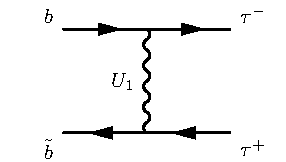
\includegraphics[width=.9\linewidth,height=.5\linewidth]{non-res_vector.pdf}
	\end{center}
	\begin{equation}
		\mathcal{M}_{U_1} \sim \frac{1}{t-m_{U_1}^2 + i m_{U_1} \Gamma_{U_1}},
	\end{equation}
\end{minipage}
\hfill
\begin{minipage}{.48\linewidth}
	Resonant Production (neutral bosons)
	\begin{center}
		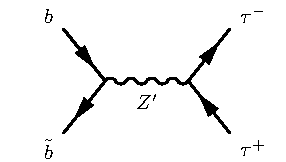
\includegraphics[width=.9\linewidth,height=.5\linewidth]{DY.pdf}
	\end{center}
	\begin{equation}
		\mathcal{M}_{Z'} \sim \frac{1}{s-m_{Z'}^2 + i m_{Z'} \Gamma_{Z'}},
	\end{equation}
\end{minipage}
so the interference has the form
		\begin{equation}\notag
				\sim \frac{ m_{LQ}m_{Z'}\Gamma_{LQ}\Gamma_{Z'}- (t-m_{LQ}^2)(s-m_{Z'}^2)}{\left[
						(t-m_{LQ}^2)^2 + m_{LQ}^2\Gamma_{LQ}^2
				\right]
				\left[
						(s-m_{Z'}^2)^2 + m_{Z'}^2\Gamma_{Z'}^2
				\right]}.
		\end{equation}
\end{frame}

\begin{frame}{Interference with a $Z'$ vector boson}
	\begin{equation*}
		% \mathrm{RKI}
		% 			=\frac{1}{\sigma_{ LQ+Z'}}
					\dv{m}\left[
							\sigma_{ LQ+Z'}-\left(\sigma_{ LQ} +\sigma_{Z'}
							\vphantom{\frac{1}2}
							\right)
							\right]
							\sim \frac{g_{z'}g_{U}}{s}\frac{ m_{LQ}m_{Z'}\Gamma_{LQ}\Gamma_{Z'}- (t-m_{LQ}^2)(s-m_{Z'}^2)}{\left[
					(t-m_{LQ}^2)^2 + m_{LQ}^2\Gamma_{LQ}^2
			\right]
			\left[
					(s-m_{Z'}^2)^2 + m_{Z'}^2\Gamma_{Z'}^2
			\right]}.
	\end{equation*}

	\begin{center}
		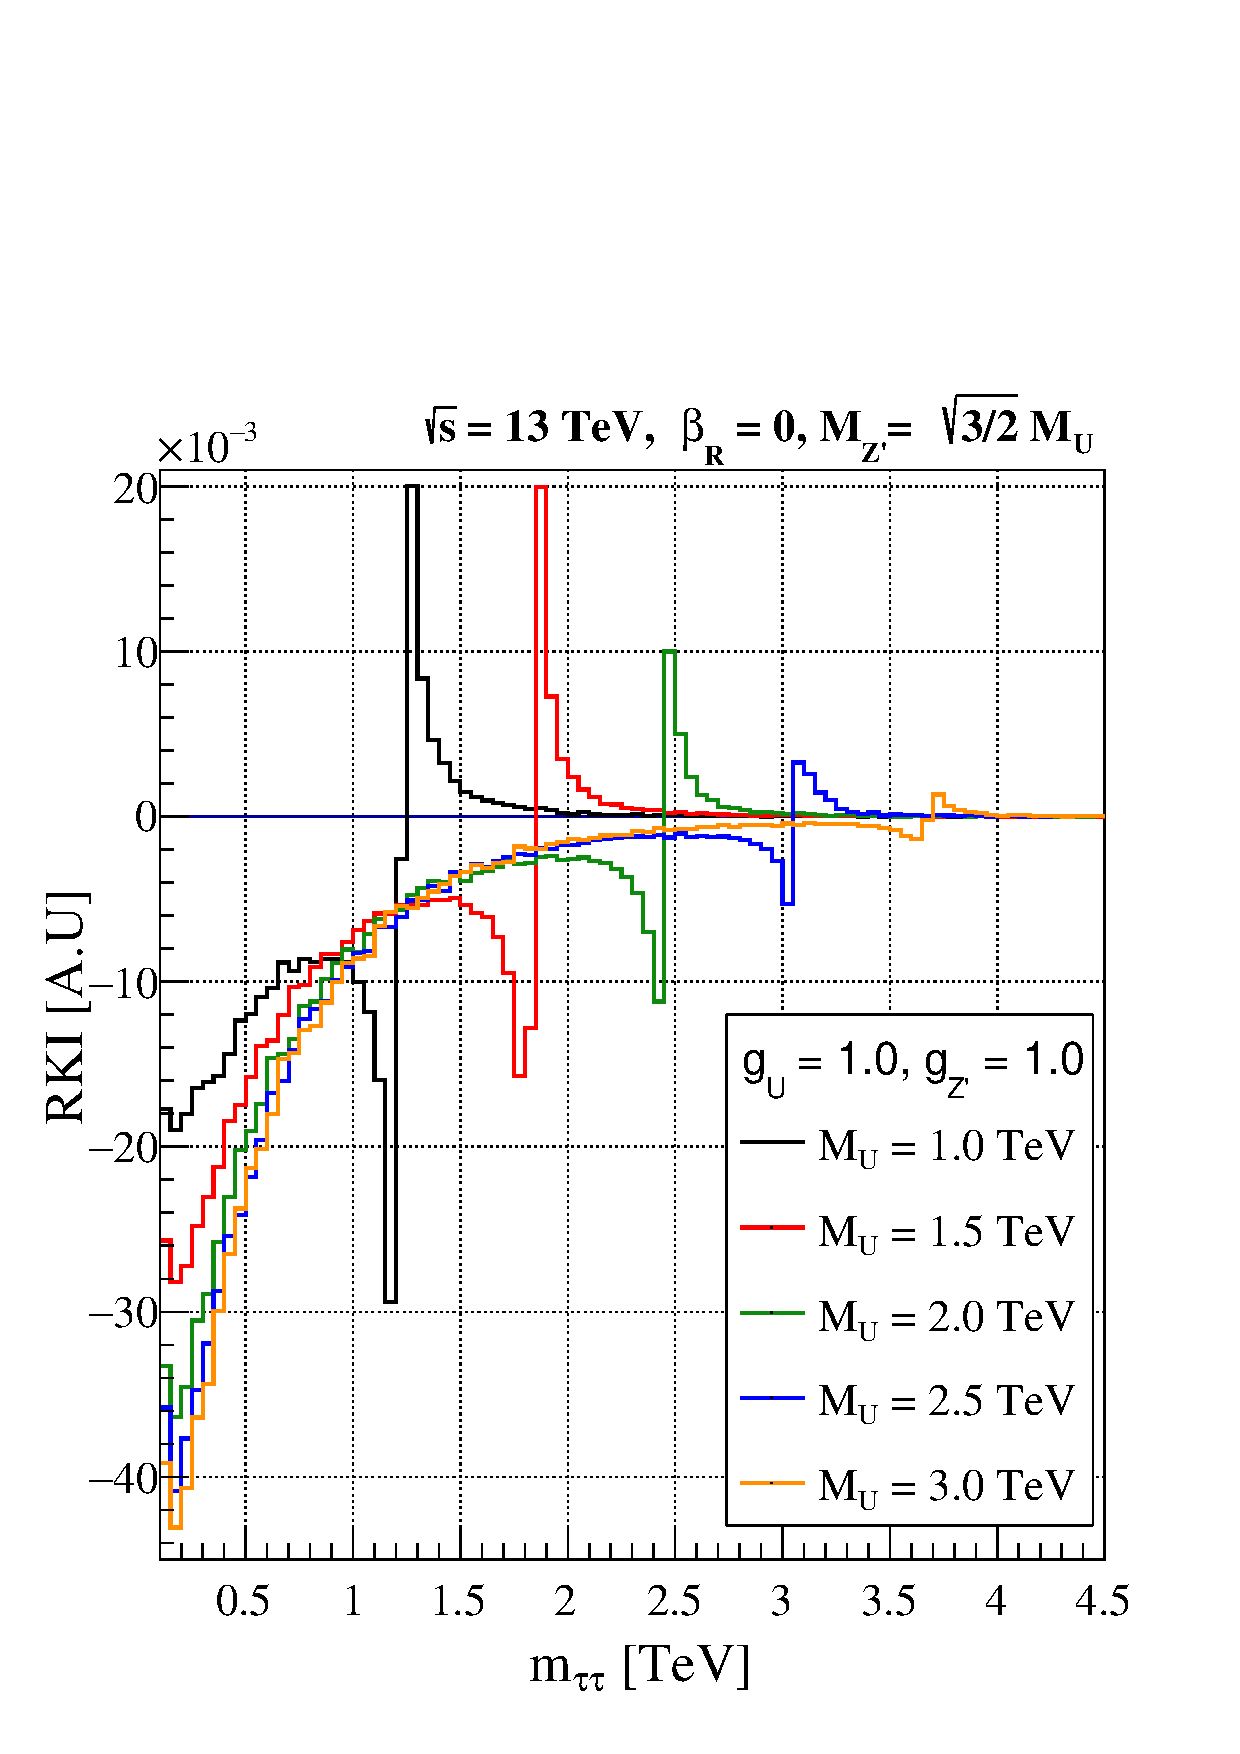
\includegraphics[width=.45\linewidth]{../2023_paper/Kinematic_Interference_gu_1.0_gzp_1.0_zp_upper_limit_woRHC.pdf}
		\hfill
		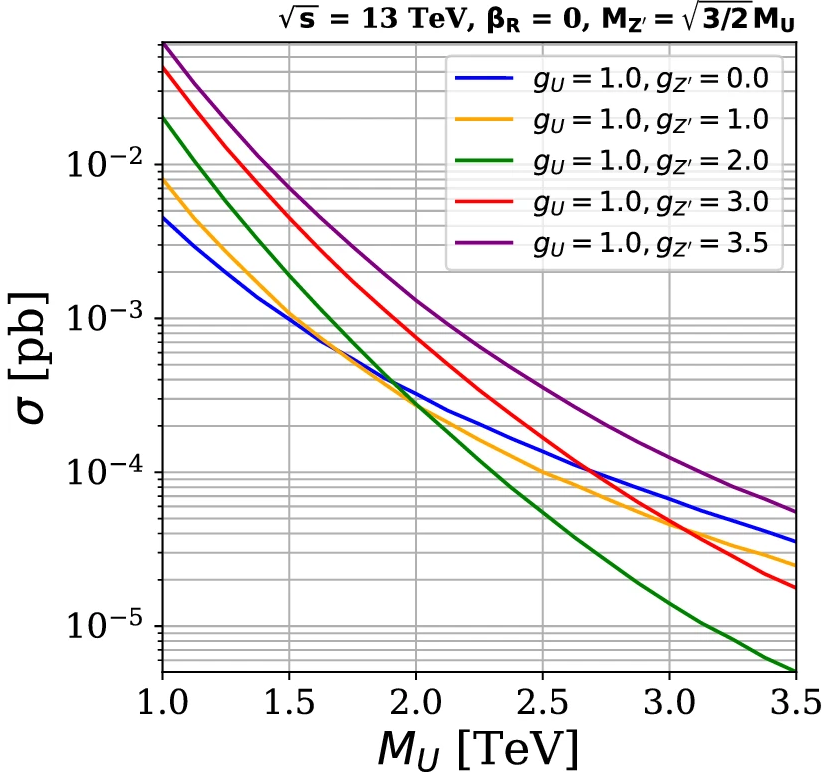
\includegraphics[width=.53\linewidth]{xs_interference.png}
	\end{center}
\end{frame}

\begin{frame}{Effects on the Sensitivity reach}
	
	\begin{center}
		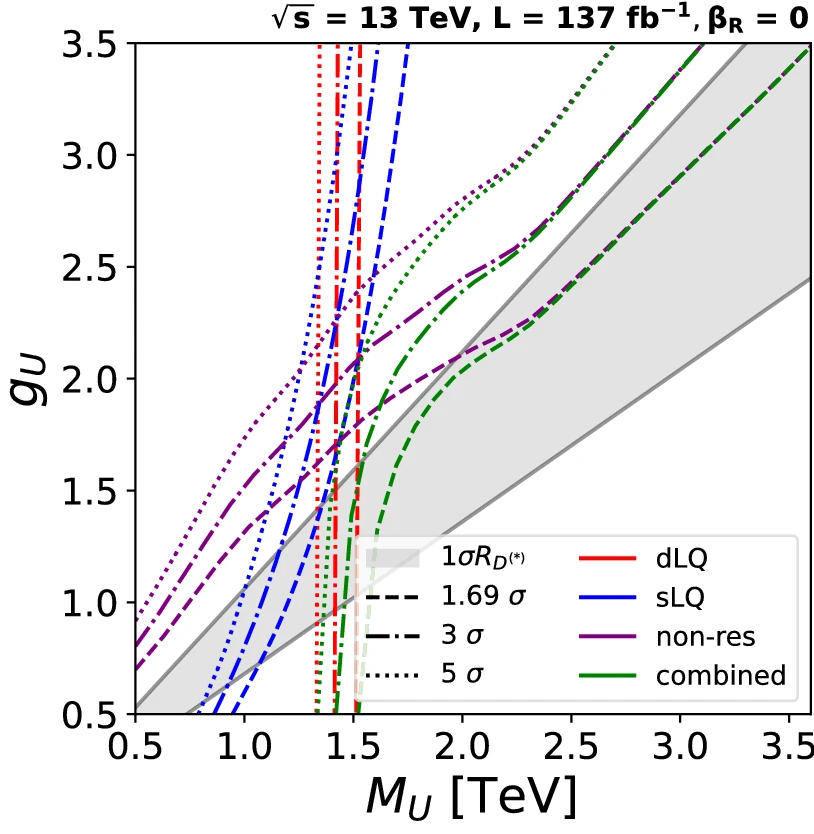
\includegraphics[width=.48\linewidth]{reach_wo_interference.png}
		\hfill
		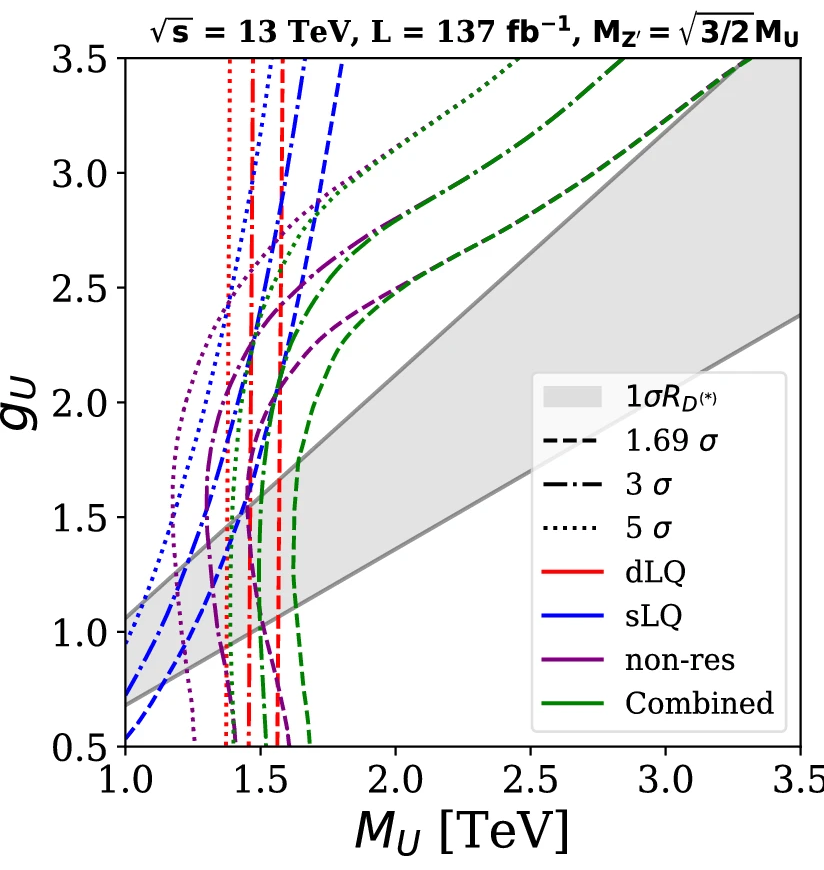
\includegraphics[width=.48\linewidth]{reach_w_interference.png}
	\end{center}
	
	
\end{frame}
\section{Final Remarks}
\begin{frame}{Final Remarks}
	\begin{itemize}
		\item We showed that LFV could be a window to new physics that could be explored at the LHC in searches with final states with $tau$ leptons. 
		\vfill
		\item It is necessary to consider possible interferences when looking for excesses in the ditaus channel that can significantly affect the sensitivity of the different parameter spaces.
		\vfill
		\item Different models, in particular gauge models, have compressed mass sectors of newly physical particles that can be extremely susceptible to interference in different production mechanisms.
		\vfill
		\item Fingerprints in the two-taus channel can inherit information from the spin of the new physics mediator, so polarization studies of each model and the associated interference effects may also be relevant.
	\end{itemize}
\end{frame}


\end{document}